% GENERATED by tools/make_results.py -- do not edit by hand.
\begin{figure}[t]
\centering
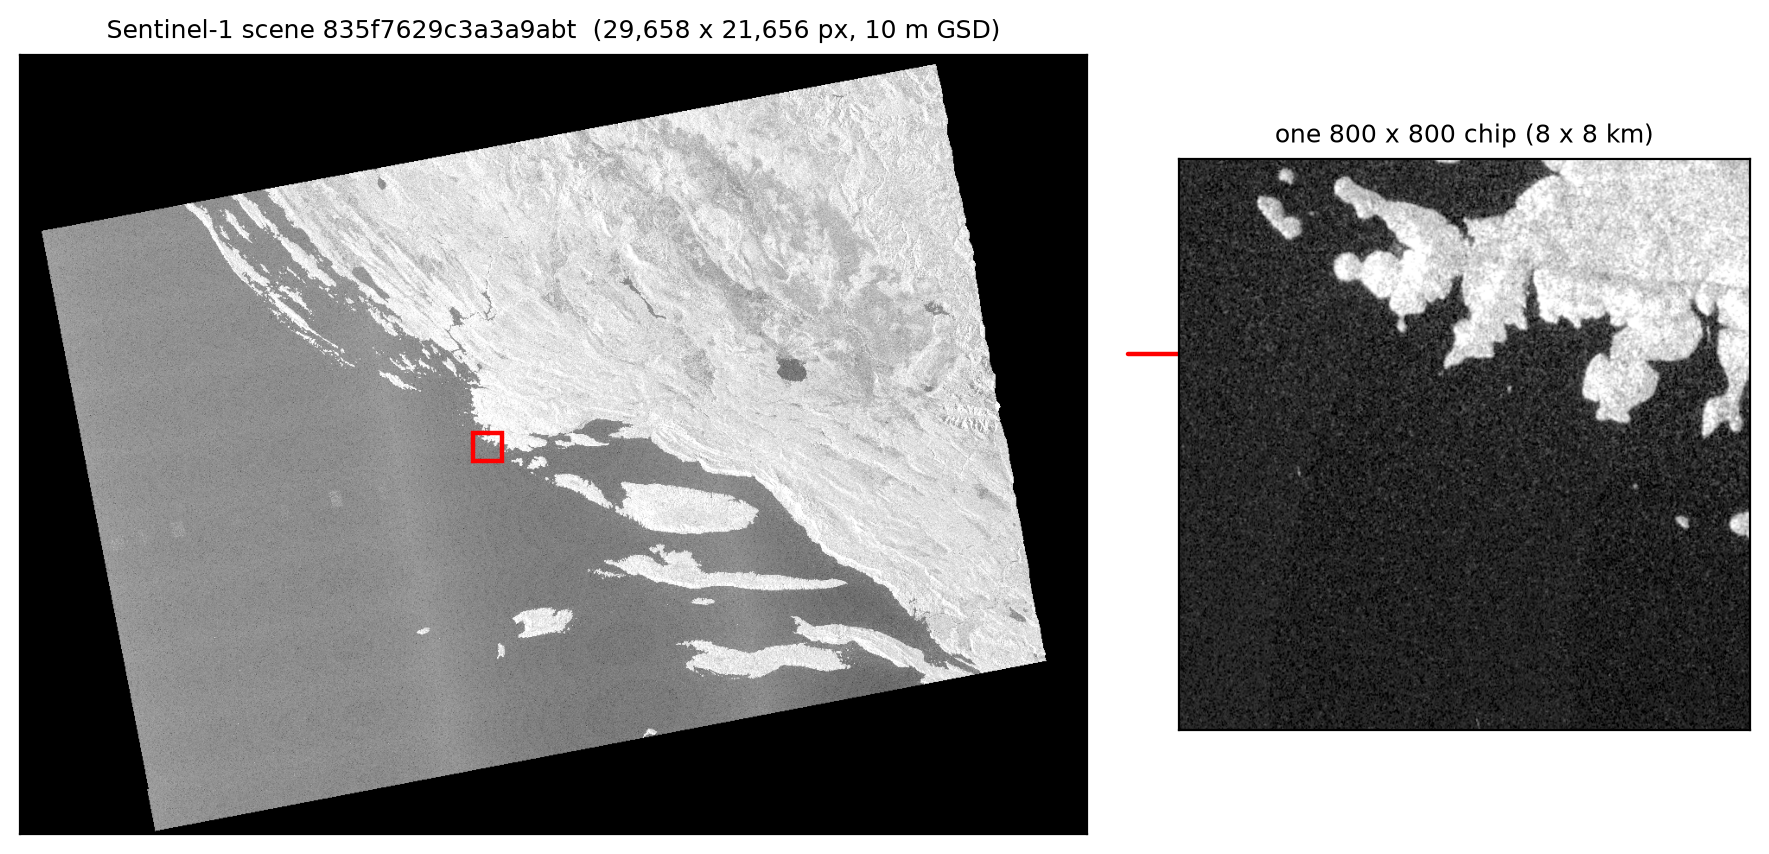
\includegraphics[width=0.82\textwidth]{figures/scene_context}\\[4pt]
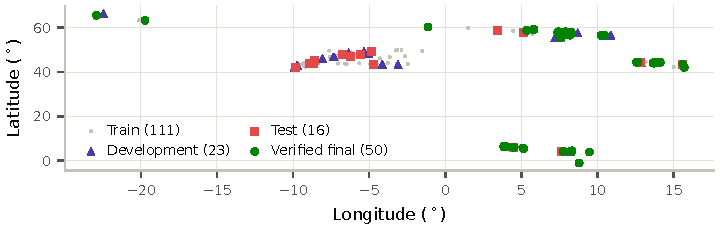
\includegraphics[width=\textwidth]{figures/scene_map}
\caption{Study data. Top: scale context for one study scene, a full
Sentinel-1 ground-range-detected scene ($29{,}658\times21{,}656$ pixels at
10 m spacing) and the single $800\times800$ chip ($8\times8$ km) marked by
the red box; vessels occupy only a few pixels at this scale. Bottom: scene
centroids of the frozen splits, computed from the label records; Sentinel-1
revisits place held-out scenes near training scenes, which is why
Sect.~\ref{sec:data-evaluation} reports in-region generalization.}
\label{fig:study-data}
\end{figure}
